% questions.tex —— 2022 年·全国乙卷·文科 · 题目内容片段（无答案）
% 由 tools/generate_projects.py 依来源总账自 2022/2022_数学真题_全国乙文_试题.md 生成，勿手改（改源 MD 后重跑）


\gkpart{一、单选题}

\begin{question}
\gkti{1}集合 $M=\{2,4,6,8,10\}$，$N=\{x\mid-1<x<6\}$，则 $M\cap N=$\mbox{（　　）}

\begin{gkopts}(4)
\task A．$\{2,4\}$
\task B．$\{2,4,6\}$
\task C．$\{2,4,6,8\}$
\task D．$\{2,4,6,8,10\}$
\end{gkopts}

\end{question}
\begin{question}
\gkti{2}设 $(1+2\mathrm i)a+b=2\mathrm i$，其中 $a,b$ 为实数，则\mbox{（　　）}

\begin{gkopts}(4)
\task A．$a=1,b=-1$
\task B．$a=1,b=1$
\task C．$a=-1,b=1$
\task D．$a=-1,b=-1$
\end{gkopts}

\end{question}
\begin{question}
\gkti{3}已知向量 $\boldsymbol a=(2,1)$，$\boldsymbol b=(-2,4)$，则 $\lvert\boldsymbol a-\boldsymbol b\rvert=$\mbox{（　　）}

\begin{gkopts}(4)
\task A．$2$
\task B．$3$
\task C．$4$
\task D．$5$
\end{gkopts}

\end{question}
\begin{question}
\gkti{4}分别统计了甲、乙两位同学 $16$ 周的各周课外体育运动时长（单位：h），得到如下茎叶图：

\begin{center}
\begin{tabular}{cll}
\toprule
茎 & 甲（叶） & 乙（叶） \\
\midrule
5 & 6，1 & — \\
6 & 8，5，3，0 & 3 \\
7 & 7，5，3，2 & 4，6 \\
8 & 6，4，2，1 & 1，2，2，5，6，6，6，6 \\
9 & 4，2 & 0，2，3，8 \\
10 & — & 1 \\
\bottomrule
\end{tabular}
\end{center}

则下列结论中错误的是\mbox{（　　）}

\begin{gkopts}(1)
\task A．甲同学周课外体育运动时长的样本中位数为 $7.4$
\task B．乙同学周课外体育运动时长的样本平均数大于 $8$
\task C．甲同学周课外体育运动时长大于 $8$ 的概率的估计值大于 $0.4$
\task D．乙同学周课外体育运动时长大于 $8$ 的概率的估计值大于 $0.6$
\end{gkopts}

\end{question}
\begin{question}
\gkti{5}若 $x,y$ 满足约束条件
\nopagebreak[4]
\[
\begin{cases}
x+y\ge 2,\\
x+2y\le 4,\\
y\ge 0,
\end{cases}
\]
则 $z=2x-y$ 的最大值是\mbox{（　　）}

\begin{gkopts}(4)
\task A．$-2$
\task B．$4$
\task C．$8$
\task D．$12$
\end{gkopts}

\end{question}
\begin{question}
\gkti{6}设 $F$ 为抛物线 $C:y^2=4x$ 的焦点，点 $A$ 在 $C$ 上，点 $B(3,0)$。若 $\lvert AF\rvert=\lvert BF\rvert$，则 $\lvert AB\rvert=$\mbox{（　　）}

\begin{gkopts}(4)
\task A．$2$
\task B．$2\sqrt2$
\task C．$3$
\task D．$3\sqrt2$
\end{gkopts}

\Needspace{0.4\textheight}
\end{question}
\begin{question}
\gkti{7}执行如图的程序框图，输出的 $n=$\mbox{（　　）}

图示转录：开始；输入 $a=1,b=1,n=1$；依次执行 $b=b+2a$、$a=b-a,\ n=n+1$；判断 $\left|\dfrac{b^2}{a^2}-2\right|<0.01$。若“是”，输出 $n$ 并结束；若“否”，返回执行 $b=b+2a$。
\nopagebreak[4]
\begin{center}\begin{tikzpicture}[>=stealth,thick,every node/.style={font=\small}]
\node[draw,rounded corners,minimum width=1.2cm,minimum height=.55cm] (start) at (0,0) {开始};
\node[minimum width=3.7cm,minimum height=.65cm] (input) at (0,-1.05) {输入 $a=1,b=1,n=1$};
\draw (-1.45,-.725)--(1.85,-.725)--(1.45,-1.375)--(-1.85,-1.375)--cycle;
\node[draw,minimum width=2.6cm,minimum height=.65cm] (bupd) at (0,-2.1) {$b=b+2a$};
\node[draw,minimum width=3.8cm,minimum height=.65cm] (anupd) at (0,-3.15) {$a=b-a,\quad n=n+1$};
\coordinate (testtop) at (0,-3.9);
\coordinate (testright) at (2.7,-4.55);
\coordinate (testbottom) at (0,-5.2);
\coordinate (testleft) at (-2.7,-4.55);
\draw (testtop)--(testright)--(testbottom)--(testleft)--cycle;
\node at (0,-4.55) {$\left|\dfrac{b^2}{a^2}-2\right|<0.01$};
\node[minimum width=2cm,minimum height=.65cm] (out) at (0,-6.05) {输出 $n$};
\draw (-.7,-5.725)--(1,-5.725)--(.7,-6.375)--(-1,-6.375)--cycle;
\node[draw,rounded corners,minimum width=1.2cm,minimum height=.55cm] (end) at (0,-7.05) {结束};
\draw[->] (start)--(input);
\draw[->] (input)--(bupd);
\draw[->] (bupd)--(anupd);
\draw[->] (anupd.south)--(testtop);
\draw[->] (testbottom)--node[right]{是}(out);
\draw[->] (out)--(end);
\draw[->] (testleft)--node[above]{否}(-3.2,-4.55)|-(bupd.west);
\end{tikzpicture}
\end{center}
\nopagebreak[4]
\begin{gkopts}(4)
\task A．$3$
\task B．$4$
\task C．$5$
\task D．$6$
\end{gkopts}

\Needspace{0.4\textheight}
\end{question}
\begin{question}
\gkti{8}如图是下列四个函数中的某个函数在区间 $[-3,3]$ 上的大致图象，则该函数是\mbox{（　　）}

图示转录：直角坐标系标出 $x=-3,1,3$ 与 $y=1$；曲线在左侧高于横轴，向下经过负值后过原点，在右侧升至正峰，再降至横轴以下。
\nopagebreak[4]
\begin{center}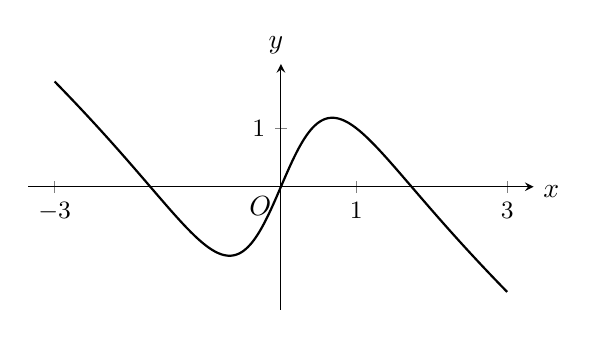
\begin{tikzpicture}
\begin{axis}[
  axis lines=middle,
  xmin=-3.35,xmax=3.35,
  ymin=-2.1,ymax=2.1,
  width=8cm,height=4.7cm,
  xtick={-3,0,1,3},
  xticklabels={$-3$,$O$,$1$,$3$},
  ytick={1},
  xlabel={$x$},ylabel={$y$},
  xlabel style={at={(axis description cs:1,.48)},anchor=west},
  ylabel style={at={(axis description cs:.49,1)},anchor=south},
  tick label style={font=\small},
  clip=true
]
\addplot[black,thick,samples=301,domain=-3:3] {(-x^3+3*x)/(x^2+1)};
\node[below left] at (axis cs:0,0) {$O$};
\end{axis}
\end{tikzpicture}
\end{center}
\nopagebreak[4]
\begin{gkopts}(2)
\task A．$y=\dfrac{-x^3+3x}{x^2+1}$
\task B．$y=\dfrac{x^3-x}{x^2+1}$
\task C．$y=\dfrac{2x\cos x}{x^2+1}$
\task D．$y=\dfrac{2\sin x}{x^2+1}$
\end{gkopts}

\end{question}
\begin{question}
\gkti{9}在正方体 $ABCD-A_1B_1C_1D_1$ 中，$E,F$ 分别为 $AB,BC$ 的中点，则\mbox{（　　）}

\begin{gkopts}(2)
\task A．平面 $B_1EF\perp$ 平面 $BDD_1$
\task B．平面 $B_1EF\perp$ 平面 $A_1BD$
\task C．平面 $B_1EF\parallel$ 平面 $A_1AC$
\task D．平面 $B_1EF\parallel$ 平面 $A_1C_1D$
\end{gkopts}

\end{question}
\begin{question}
\gkti{10}已知等比数列 $\{a_n\}$ 的前 $3$ 项和为 $168$，$a_2-a_5=42$，则 $a_6=$\mbox{（　　）}

\begin{gkopts}(4)
\task A．$14$
\task B．$12$
\task C．$6$
\task D．$3$
\end{gkopts}

\end{question}
\begin{question}
\gkti{11}函数 $f(x)=\cos x+(x+1)\sin x+1$ 在区间 $[0,2\pi]$ 的最小值、最大值分别为\mbox{（　　）}

\begin{gkopts}(2)
\task A．$\left(-\dfrac\pi2,\dfrac\pi2\right)$
\task B．$\left(-\dfrac{3\pi}2,\dfrac\pi2\right)$
\task C．$\left(-\dfrac\pi2,\dfrac\pi2+2\right)$
\task D．$\left(-\dfrac{3\pi}2,\dfrac\pi2+2\right)$
\end{gkopts}

\end{question}
\begin{question}
\gkti{12}已知球 $O$ 的半径为 $1$，四棱锥的顶点为 $O$，底面的四个顶点均在球 $O$ 的球面上，则当该四棱锥的体积最大时，其高为\mbox{（　　）}

\begin{gkopts}(2)
\task A．$\dfrac13$
\task B．$\dfrac12$
\task C．$\dfrac{\sqrt3}{3}$
\task D．$\dfrac{\sqrt2}{2}$
\end{gkopts}

\end{question}
\gkpart{二、填空题}

\begin{question}
\gkti{13}记 $S_n$ 为等差数列 $\{a_n\}$ 的前 $n$ 项和。若 $2S_3=3S_2+6$，则公差 $d=$ \gkblank{}。

\end{question}
\begin{question}
\gkti{14}从甲、乙等 $5$ 名同学中随机选 $3$ 名参加社区服务工作，则甲、乙都入选的概率为 \gkblank{}。

\end{question}
\begin{question}
\gkti{15}过四点 $(0,0),(4,0),(-1,1),(4,2)$ 中的三点的一个圆的方程为 \gkblank{}。

\end{question}
\begin{question}
\gkti{16}若函数
\nopagebreak[4]
\[
f(x)=\ln\left|a+\frac{1}{1-x}\right|+b
\]
是奇函数，则 $a=$ \gkblank{}，$b=$ \gkblank{}。

\end{question}
\gkpart{三、解答题}

\begin{question}
\gkti{17}记 $\triangle ABC$ 的内角 $A,B,C$ 的对边分别为 $a,b,c$。已知
\nopagebreak[4]
\[
\sin C\sin(A-B)=\sin B\sin(C-A).
\]

(1) 若 $A=2B$，求 $C$；

(2) 证明：$2a^2=b^2+c^2$。

\Needspace{0.4\textheight}
\end{question}
\begin{question}
\gkti{18}如图，四面体 $ABCD$ 中，$AD\perp CD$，$AD=CD$，$\angle ADB=\angle BDC$，$E$ 为 $AC$ 的中点。

图示转录：四面体顶点为 $A,B,C,D$；$E$ 标在 $AC$ 上，$F$ 标在 $BD$ 上；实线、虚线区分可见与隐藏棱。
\nopagebreak[4]
\begin{center}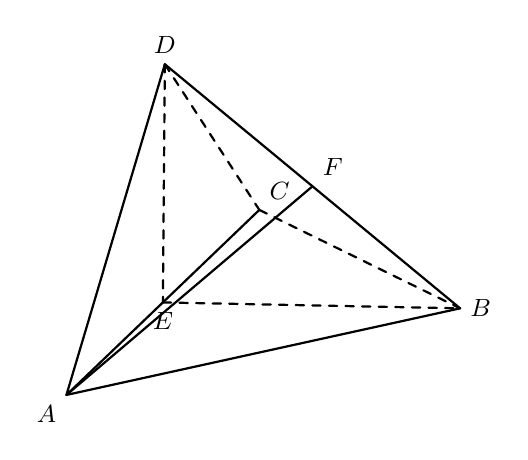
\begin{tikzpicture}[thick,line cap=round,line join=round,every node/.style={font=\small}]
\coordinate (A) at (0,0);
\coordinate (B) at (5,1.1);
\coordinate (D) at (1.25,4.2);
\coordinate (C) at (2.45,2.35);
\coordinate (E) at (1.225,1.175);
\coordinate (F) at (3.125,2.65);
\draw (A)--(D)--(B)--(A);
\draw (A)--(C);
\draw[dashed] (D)--(C);
\draw[dashed] (C)--(B);
\draw[dashed] (D)--(E);
\draw[dashed] (E)--(B);
\draw (A)--(F);
\node[below left] at (A) {$A$};
\node[right] at (B) {$B$};
\node[above] at (D) {$D$};
\node[above right] at (C) {$C$};
\node[below] at (E) {$E$};
\node[above right] at (F) {$F$};
\end{tikzpicture}
\end{center}
\nopagebreak[4]
(1) 证明：平面 $BED\perp$ 平面 $ACD$；

(2) 设 $AB=BD=2$，$\angle ACB=60^\circ$，点 $F$ 在 $BD$ 上，当 $\triangle AFC$ 的面积最小时，求三棱锥 $F-ABC$ 的体积。

\end{question}
\begin{question}
\gkti{19}某地经过多年的环境治理，已将荒山改造成了绿水青山。为估计林区某种树木的总材积量，随机选取了 $10$ 棵这种树木，测量每棵树的根部横截面积（单位：$\mathrm m^2$）和材积量（单位：$\mathrm m^3$），得到如下数据：

\begin{center}
\begingroup\setlength{\tabcolsep}{4pt}
\begin{tabular}{lrrrrrrrrrrr}
\toprule
样本号 $i$ & 1 & 2 & 3 & 4 & 5 & 6 & 7 & 8 & 9 & 10 & 总和 \\
\midrule
根部横截面积 $x_i$ & 0.04 & 0.06 & 0.04 & 0.08 & 0.08 & 0.05 & 0.05 & 0.07 & 0.07 & 0.06 & 0.6 \\
材积量 $y_i$ & 0.25 & 0.40 & 0.22 & 0.54 & 0.51 & 0.34 & 0.36 & 0.46 & 0.42 & 0.40 & 3.9 \\
\bottomrule
\end{tabular}
\endgroup
\end{center}

\Needspace{5\baselineskip}
并计算得
\nopagebreak[4]
\[
\sum_{i=1}^{10}x_i^2=0.038,\qquad
\sum_{i=1}^{10}y_i^2=1.6158,\qquad
\sum_{i=1}^{10}x_iy_i=0.2474.
\]

(1) 估计该林区这种树木平均一棵的根部横截面积与平均一棵的材积量；

(2) 求该林区这种树木的根部横截面积与材积量的样本相关系数（精确到 $0.01$）；

(3) 现测量了该林区所有这种树木的根部横截面积，并得到所有这种树木的根部横截面积总和为 $186\ \mathrm m^2$。已知树木的材积量与其根部横截面积近似成正比。利用以上数据给出该林区这种树木的总材积量的估计值。

\Needspace{5\baselineskip}
附：相关系数
\nopagebreak[4]
\[
r=\frac{\sum_{i=1}^{n}(x_i-\bar x)(y_i-\bar y)}
{\sqrt{\sum_{i=1}^{n}(x_i-\bar x)^2\sum_{i=1}^{n}(y_i-\bar y)^2}},
\qquad \sqrt{1.896}\approx1.377.
\]

\end{question}
\begin{question}
\gkti{20}已知函数
\nopagebreak[4]
\[
f(x)=ax-\frac1x-(a+1)\ln x.
\]

(1) 当 $a=0$ 时，求 $f(x)$ 的最大值；

(2) 若 $f(x)$ 恰有一个零点，求 $a$ 的取值范围。

\end{question}
\begin{question}
\gkti{21}已知椭圆 $E$ 的中心为坐标原点，对称轴为 $x$ 轴、$y$ 轴，且过 $A(0,-2)$，$B\left(\dfrac32,-1\right)$ 两点。

(1) 求 $E$ 的方程；

(2) 设过点 $P(1,-2)$ 的直线交 $E$ 于 $M,N$ 两点，过 $M$ 且平行于 $x$ 轴的直线与线段 $AB$ 交于点 $T$，点 $H$ 满足 $\overrightarrow{MT}=\overrightarrow{TH}$。证明：直线 $HN$ 过定点。

\end{question}
\begin{question}
\gkti{22}在直角坐标系 $xOy$ 中，曲线 $C$ 的参数方程为
\nopagebreak[4]
\[
\begin{cases}
x=\sqrt3\cos 2t,\\
y=2\sin t
\end{cases}
\qquad(t\text{ \text{为参数}}).
\]
\Needspace{5\baselineskip}
以坐标原点为极点，$x$ 轴正半轴为极轴建立极坐标系，已知直线 $l$ 的极坐标方程为
\nopagebreak[4]
\[
\rho\sin\left(\theta+\frac\pi3\right)+m=0.
\]

(1) 写出 $l$ 的直角坐标方程；

(2) 若 $l$ 与 $C$ 有公共点，求 $m$ 的取值范围。

\end{question}
\begin{question}
\gkti{23}已知 $a,b,c$ 都是正数，且
\nopagebreak[4]
\[
a^{3/2}+b^{3/2}+c^{3/2}=1,
\]
证明：

(1) $abc\le\dfrac19$；

(2) $\dfrac{a}{b+c}+\dfrac{b}{a+c}+\dfrac{c}{a+b}\le\dfrac{1}{2\sqrt{abc}}$。

\end{question}